\documentclass[landscape, 12pt]{beamer}

\usetheme{Madrid}
\usecolortheme{default}

\usepackage[utf8]{inputenc}
\usepackage[T1]{fontenc}
\usepackage[brazil]{babel}
\usepackage{graphicx}
\usepackage{amsmath,amssymb}
\usepackage{wasysym}
\usepackage{float}
\usepackage{xcolor}
\usepackage{hyperref}
\usepackage{tabularx}

\title{Análise de Crescimento de Plantas a Partir de Fotos Semanais}
\subtitle{Plant Growth Analyzer}
\author{
    Lucas Cardoso dos Santos \\
    Lucas Miranda Mendonça Rezende
}
\institute{Universidade de São Paulo - Ribeirão Preto}
\date{2025}

% Remove barra inferior e símbolos de navegação
\setbeamertemplate{footline}{}
\setbeamertemplate{navigation symbols}{}

\begin{document}

% Slide de título
\begin{frame}
    \titlepage
\end{frame}

% Slide de sumário
\begin{frame}{Sumário}
    \begin{enumerate}
        \item Introdução
        \item Desenvolvimento
        \item Problemas
        \item Resultados
        \item Conclusão
    \end{enumerate}
\end{frame}

% Seção 1: Introdução
\begin{frame}{Introdução}
    \begin{center}
        \textbf{Agricultura Inteligente}
    \end{center}
\end{frame}

\begin{frame}{Proposta do Projeto}
    \textbf{Objetivo}: Desenvolver um método automatizado para extrair métricas de crescimento de plantas (área, altura e largura) a partir de imagens digitais
    
    \vspace{0.5cm}
    \textbf{Aplicações}:
    \begin{itemize}
        \item Criação de benchmarks científicos
        \item Estimativa de safras agrícolas
        \item Monitoramento da saúde das culturas
        \item Detecção precoce de pragas/doenças
        \item Otimização de recursos (água, fertilizantes)
    \end{itemize}
\end{frame}

% Seção 2: Desenvolvimento
\begin{frame}{Desenvolvimento}
    \begin{center}
        \textbf{Algoritmo de Processamento de Imagem}
    \end{center}
\end{frame}

\begin{frame}{Visão Geral do Pipeline}
    \begin{enumerate}
        \item \textbf{Leitura e validação} da entrada
        \item \textbf{Decodificação e pré-processamento} da imagem
        \item \textbf{Detecção de bordas} e segmentação
        \item \textbf{Identificação da região} da planta
        \item \textbf{Pós-processamento} da máscara
        \item \textbf{Extração de medidas} morfológicas
        \item \textbf{Geração da imagem} de saída
    \end{enumerate}
\end{frame}

\begin{frame}{Passo 1: Leitura e Validação}
    \textbf{Entrada}: 
    \begin{itemize}
        \item Identificador único para cada imagem
        \item Arquivo JSON com parâmetros (granularidade, limiar)
        \item Imagem codificada em base64
    \end{itemize}
    
    \vspace{0.5cm}
    \textbf{Validação}:
    \begin{itemize}
        \item Verificação da versão do Python
        \item Validação das dependências
        \item Prevenção de falhas de compatibilidade
    \end{itemize}
\end{frame}

\begin{frame}{Passo 2: Decodificação e Pré-processamento}
    \textbf{Decodificação}:
    \begin{itemize}
        \item Conversão de base64 para imagem
        \item Redimensionamento adaptativo (máx. 1024px)
    \end{itemize}
    
    \vspace{0.5cm}
    \textbf{Pré-processamento}:
    \begin{itemize}
        \item Conversão para tons de cinza
        \item Desfoque gaussiano adaptativo
        \item Realce de contraste com CLAHE
        \item Redução de ruídos e variações locais
    \end{itemize}
\end{frame}

\begin{frame}{Passo 3: Segmentação - Algoritmo Watershed}
    \textbf{Detecção de bordas}:
    \begin{itemize}
        \item Filtro de Sobel
        \item Fechamento morfológico
    \end{itemize}
    
    \vspace{0.5cm}
    \textbf{Algoritmo Watershed}:
    \begin{itemize}
        \item Interpretação da imagem como superfície topográfica
        \item Marcadores definidos em regiões de interesse
        \item Simulação de "preenchimento com água"
        \item Criação de fronteiras entre objetos
        \item Robusto para objetos conectados
    \end{itemize}
\end{frame}

\begin{frame}{Passo 4: Identificação da Planta}
    \textbf{Análise de cor em dois espaços}:
    \begin{itemize}
        \item \textbf{BGR}: modelo tradicional RGB
        \item \textbf{HSV}: separa matiz, saturação e valor
    \end{itemize}
    
    \vspace{0.5cm}
    \textbf{Critério principal}: Predominância de tons de verde
    
    \vspace{0.5cm}
    \textbf{Vantagens}:
    \begin{itemize}
        \item Robusto a variações de iluminação
        \item Adaptativo para diferentes espécies
        \item Reduz falsos positivos
    \end{itemize}
\end{frame}

\begin{frame}{Passo 5: Pós-processamento da Máscara}
    \textbf{Problemas na segmentação}:
    \begin{itemize}
        \item Buracos devido a reflexos
        \item Falhas por sombras
        \item Regiões desconectadas
    \end{itemize}
    
    \vspace{0.5cm}
    \textbf{Soluções}:
    \begin{itemize}
        \item Operações morfológicas de fechamento
        \item Preenchimento de buracos
        \item Tamanho mínimo ajustado dinamicamente
        \item Garantia de continuidade da área foliar
    \end{itemize}
\end{frame}

\begin{frame}{Passo 6: Extração de Medidas}
    \textbf{Três medidas morfológicas principais}:
    
    \vspace{0.5cm}
    \begin{itemize}
        \item \textbf{Área}: Contagem de pixels segmentados
        \item \textbf{Altura}: Regressão linear dos pontos → extensão máxima ao longo do eixo principal
        \item \textbf{Largura}: Projeção no eixo perpendicular à reta ajustada
    \end{itemize}
\end{frame}

\begin{frame}{Passo 7: Geração da Imagem de Saída}
    \textbf{Visualização dos resultados}:
    \begin{itemize}
        \item Sobreposição da máscara segmentada
        \item Linhas de medição coloridas:
        \begin{itemize}
            \item Altura em amarelo
            \item Largura em magenta
        \end{itemize}
        \item Codificação em base64 (JPEG/PNG)
    \end{itemize}
    
    \vspace{0.5cm}
    \textbf{Resultado}: Processo interpretável e transparente para o usuário
\end{frame}

% Seção 3: Problemas
\begin{frame}{Problemas Encontrados}
    \begin{center}
        \textbf{Detecção de Caules}
    \end{center}
\end{frame}

\begin{frame}{Dificuldades na Detecção de Caules}
    \textbf{Principal desafio}: Detecção automática dos caules das plantas
    
    \vspace{0.5cm}
    \textbf{Problemas identificados}:
    \begin{itemize}
        \item Grande variação de tonalidade (marrom claro a esverdeado)
        \item Sombras projetadas pelas folhas
        \item Reflexos do solo úmido
        \item Semelhança com substrato e galhos secos
        \item Muitos falsos positivos e negativos
    \end{itemize}
\end{frame}

\begin{frame}{Tentativas de Solução}
    \textbf{1. Segmentação por cor}:
    \begin{itemize}
        \item Limiares nos espaços BGR e HSV
        \item Resultado: intervalo de cor não robusto
    \end{itemize}
    
    \vspace{0.3cm}
    \textbf{2. Morfologia e geometria}:
    \begin{itemize}
        \item Transformada de Radon para estruturas lineares
        \item Resultado: resposta difusa, pouco informativa
    \end{itemize}
    
    \vspace{0.3cm}
    \textbf{3. Machine Learning}:
    \begin{itemize}
        \item Classificadores tradicionais e CNNs
        \item Resultado: baixa precisão, alta taxa de erro
    \end{itemize}
\end{frame}

\begin{frame}{Exemplos de Tentativas Frustradas}
    \begin{center}
        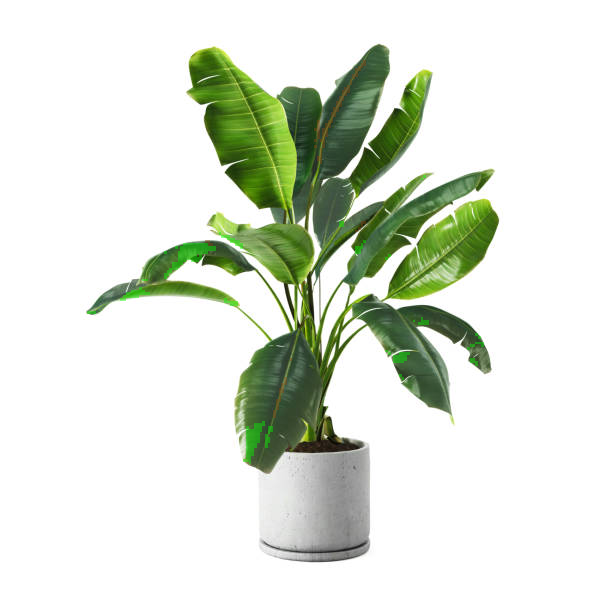
\includegraphics[height=4cm]{../figures/ml_results/attempt1.png}
        \hspace{0.2cm}
        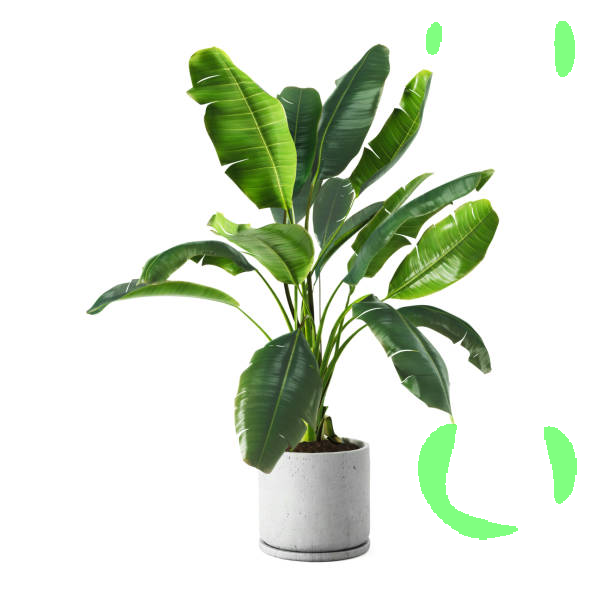
\includegraphics[height=4cm]{../figures/ml_results/attempt2.png}
        \hspace{0.2cm}
        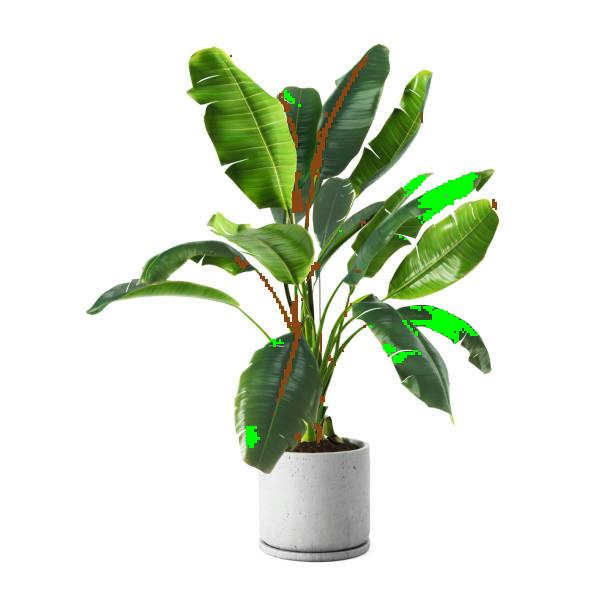
\includegraphics[height=4cm]{../figures/ml_results/attempt3.jpg}
    \end{center}
    
    \vspace{0.3cm}
    \textbf{Conclusão}: Solução final restrita à detecção de folhas
\end{frame}

% Seção 4: Resultados
\begin{frame}{Resultados}
    \begin{center}
        \textbf{Interface Gráfica Desenvolvida}
    \end{center}
\end{frame}

\begin{frame}{Tela Principal}
    \begin{center}
        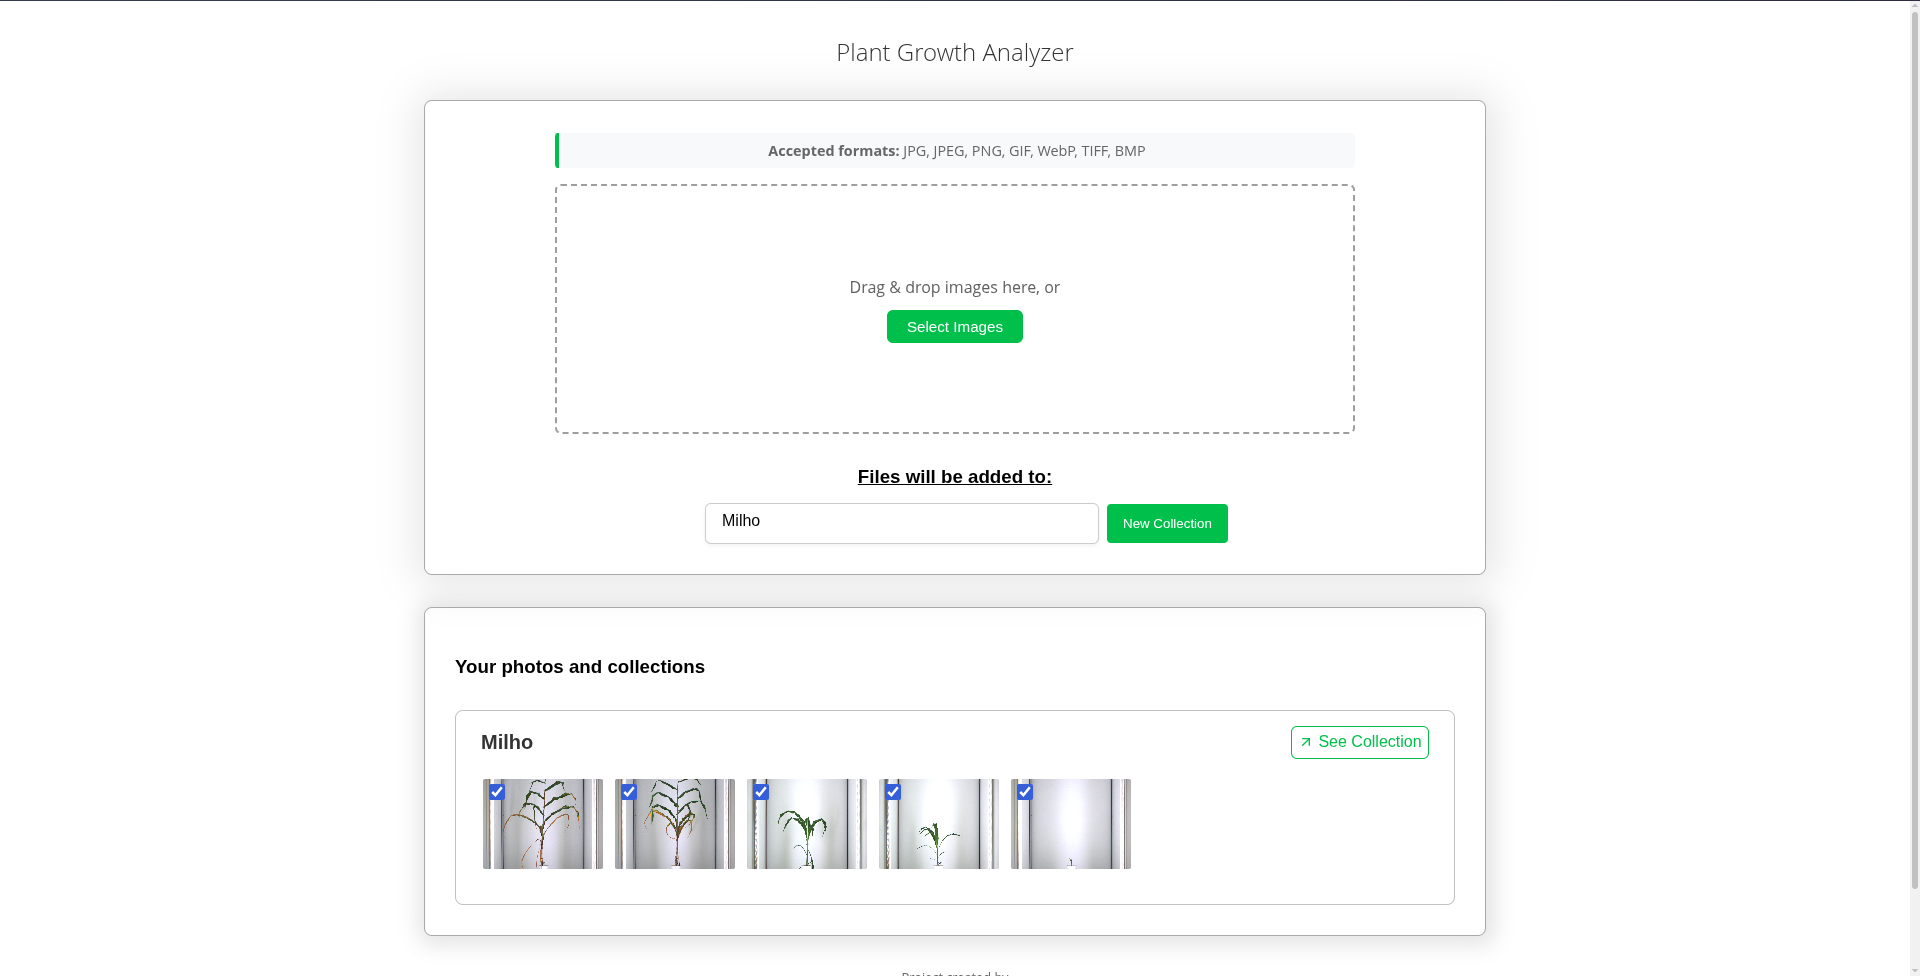
\includegraphics[width=0.9\textwidth]{../figures/screens/interface-grafica.png}
    \end{center}
\end{frame}

\begin{frame}{Visualização de Coleções}
    \begin{center}
        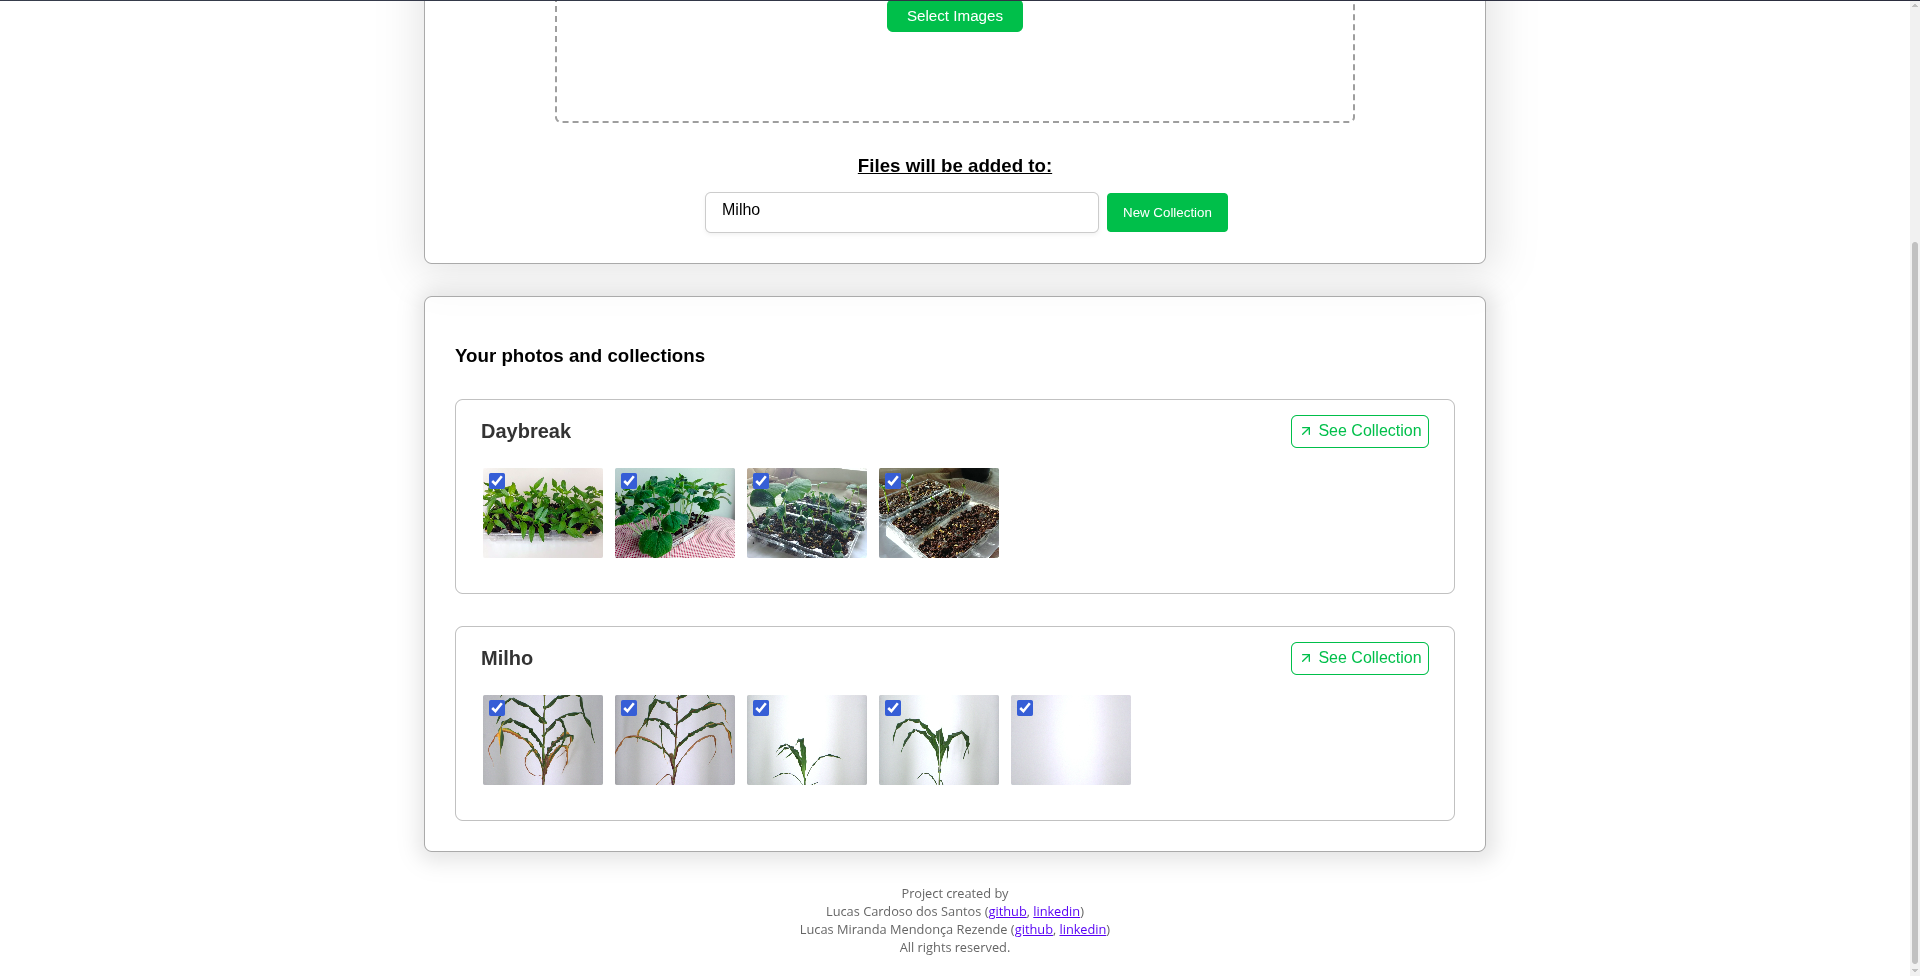
\includegraphics[width=0.9\textwidth]{../figures/screens/colecoes.png}
    \end{center}
\end{frame}

\begin{frame}{Processamento Individual}
    \begin{center}
        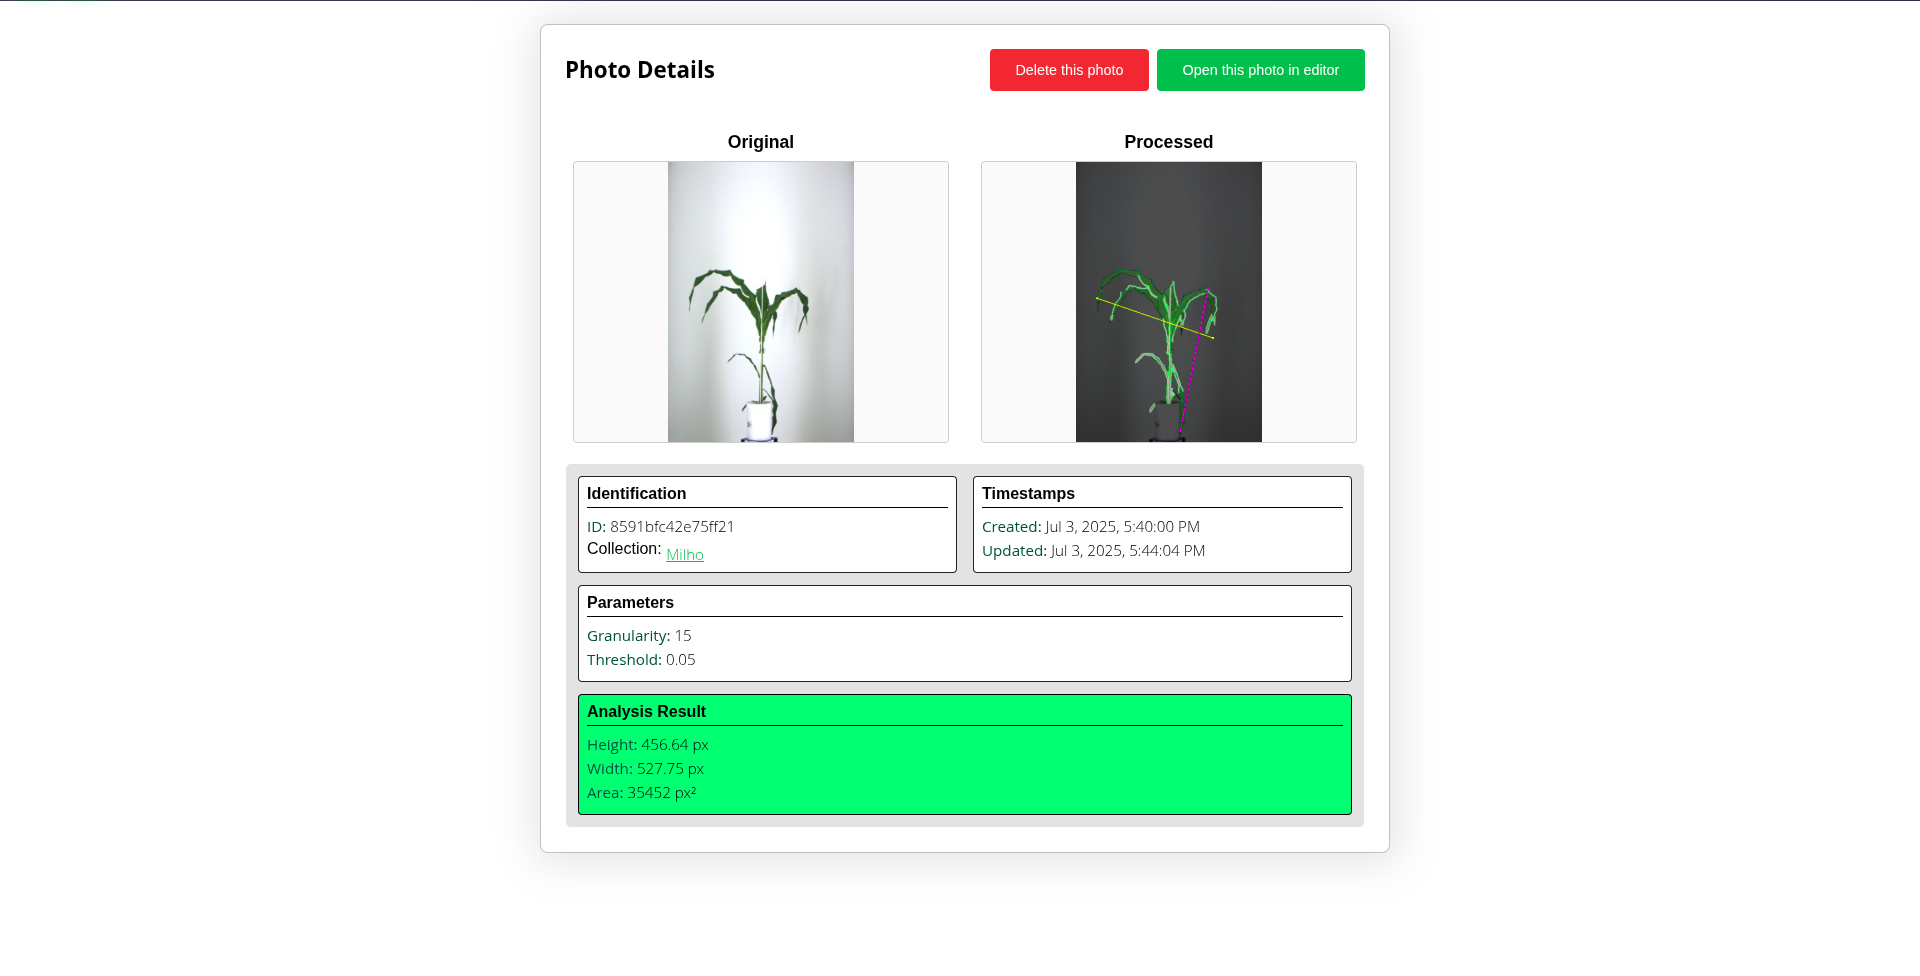
\includegraphics[width=0.9\textwidth]{../figures/screens/processamento-individual.png}
    \end{center}
\end{frame}

\begin{frame}{Gráficos de Crescimento}
    \begin{center}
        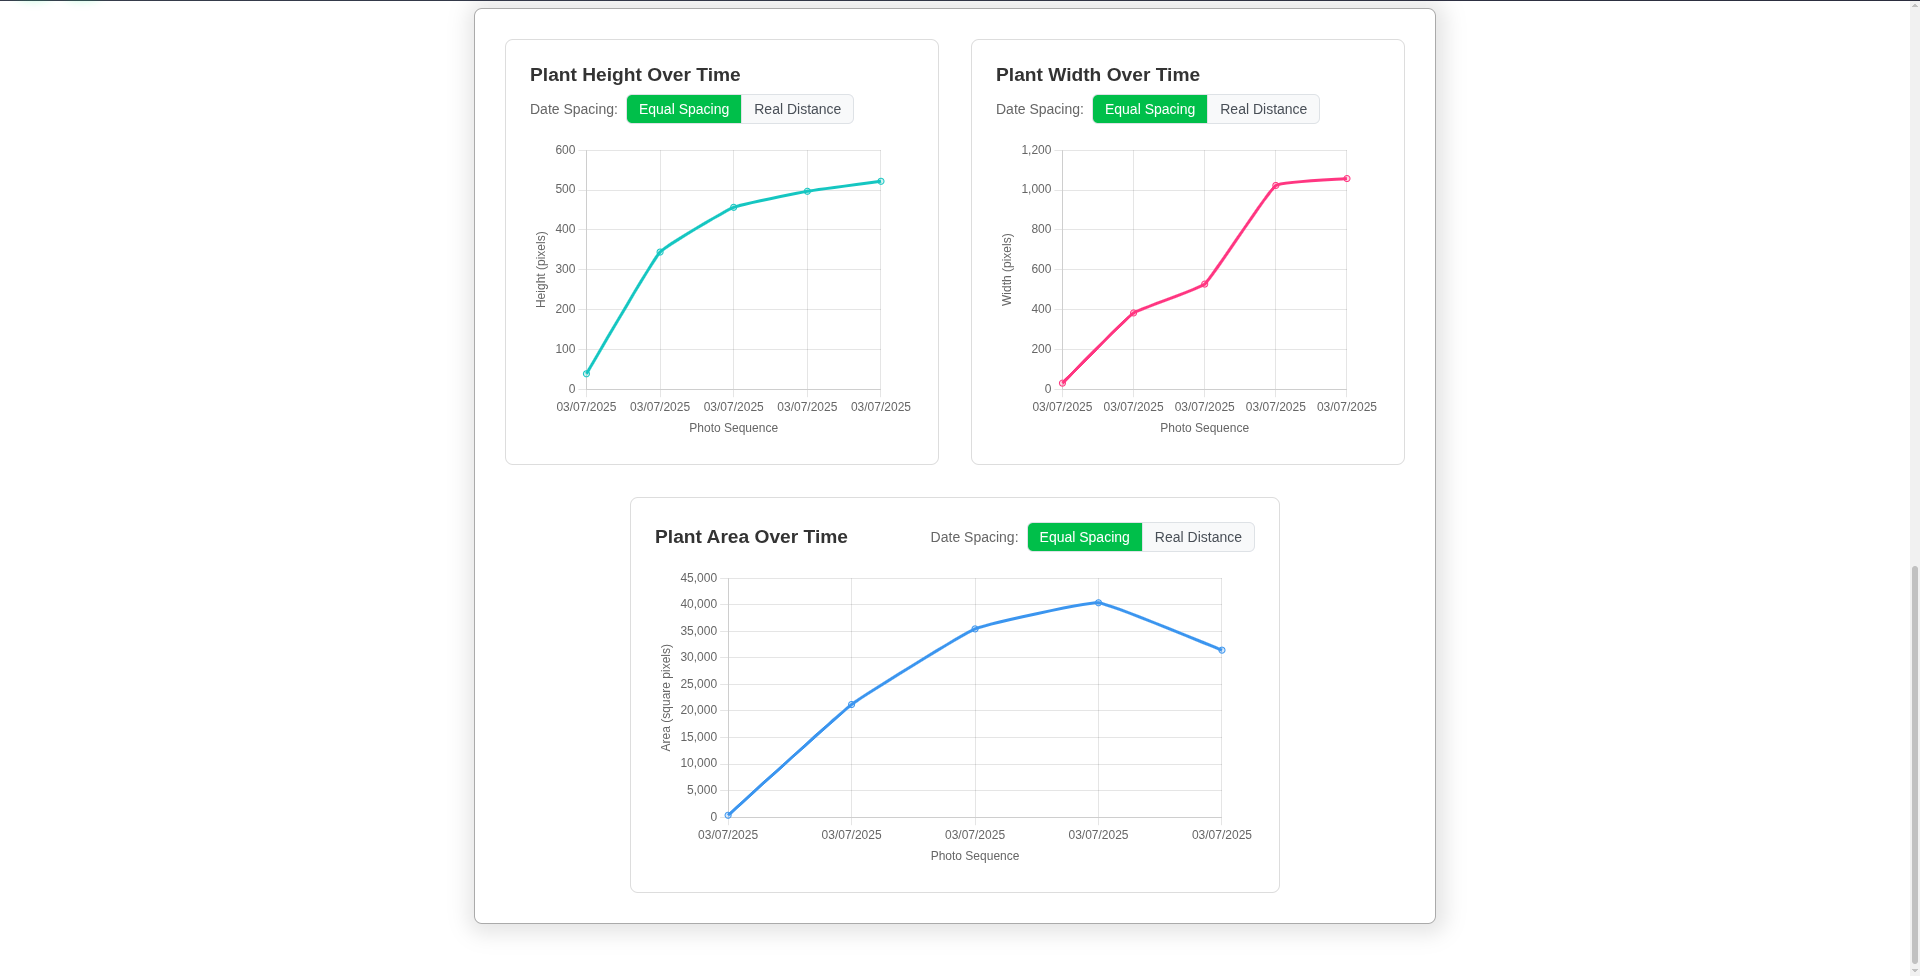
\includegraphics[width=0.9\textwidth]{../figures/screens/grafico-crescimento.png}
    \end{center}
\end{frame}

% Seção 5: Conclusão
\begin{frame}{Conclusão}
    \begin{center}
        \textbf{Avaliação da Performance}
    \end{center}
\end{frame}

\begin{frame}{Resultados Alcançados}
    \textbf{Pontos positivos}:
    \begin{itemize}
        \item Máscaras precisas para identificação de folhas
        \item Medidas morfológicas estáveis e reprodutíveis
        \item Processo transparente e confiável
        \item Interface intuitiva e eficiente
        \item Solução completa e acessível
    \end{itemize}
    
    \vspace{0.5cm}
    \textbf{Limitações}:
    \begin{itemize}
        \item Detecção de caules não implementada
        \item Conversão pixel → medidas reais não abordada
    \end{itemize}
\end{frame}

\begin{frame}{Avaliação da Performance}
    \textbf{Eficácia do sistema}:
    \begin{itemize}
        \item Segmentação robusta em diferentes condições
        \item Resistente a variações de iluminação
        \item Acompanhamento quantitativo do crescimento
        \item Adequado para pesquisa, ensino e hobby
    \end{itemize}
    
    \vspace{0.5cm}
    \textbf{Contribuição}:
    \begin{itemize}
        \item Modernização do monitoramento vegetal
        \item Democratização de técnicas de análise
        \item Automação de práticas manuais
        \item Base para futuras melhorias
    \end{itemize}
\end{frame}

\begin{frame}{}
    \vspace{0.8cm}
    \begin{center}
        \textbf{Obrigado!}
        
        \vspace{0.3cm}
        Lucas Cardoso dos Santos \\
        Lucas Miranda Mendonça Rezende
    \end{center}
\end{frame}

\end{document}

